\chapter{QM/MM Non-adiabatic Dynamics of PPV\(_3\)-NO\(_2\)}

\section{Introduction}
We further our analysis of PPV3no2 by analyzing its ultra fast excited state decay.
Recent works have analized the nonadiabatic behaviors of PPV3NO2  to the study of its na dynamics in implicit solvent. \cite{sifain2018photoexcited,dykstra2009conformational}
This type of work is useful for studying the donor acceptor functionality of this promising organic conjugated molecular in polarized solvents.
We choose methanol due to it being a common solvent with strong polarization.
We'll compare the population decay behavior to that found in strongly polar implicit solvents.

\section{Simulation Methods}

\noindent
\begin{minipage}[c]{\textwidth}
  \centering
  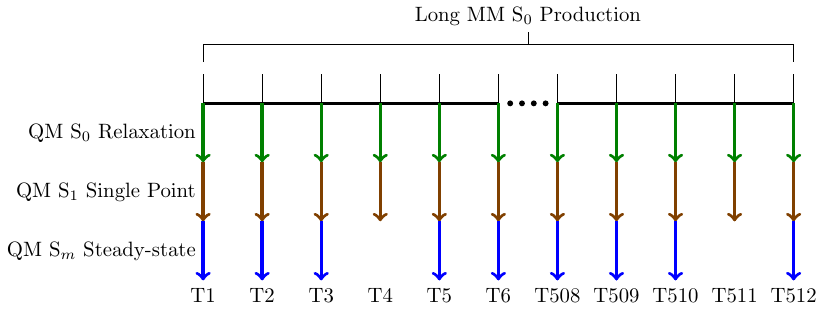
\includegraphics[width=5in]{../Paper2/scripted_diagrams/simulations-1.png}
  \captionof{figure}{Diagram of the Nonadiabatic dyanmics simulation.}
  \label{fig:nonadiabaticSimulation}
\end{minipage}\bigskip

We equilibrated the system to a temperature set to 300K. To collect a broad
enough sampling, we sampled from a 1024 ps, with a 0.5 fs time-step fully
classical trajectories using the AMBER force field. We performed a separate
trajectory for each situation combination of solute / with solvent including
whether the solvent was included in the QM calculations. We had a total of 6
separate 1024 ps classical trajectories, PPV3 in Vacuum, CH\(_3\)OH, and 5QM CH\(_3\)OH
and PPV\(_3\)-NO\(_2\) in Vacuum, CH\(_3\)OH, and 5QM CH\(_3\)OH. 1024 snapshots where taken at
1ps, 2ps .. 1024ps. We used the final frame of those tranjectories as the
initial conditions for an additional 4ps using the AM1 semiempical Hamiltonian
Born-Oppenheimer on the molecules to be included in future QM calculations to
allow the system to relax. The 4 ps timescale was determined using the
information form the previous paper. The simulations were described the Langevin
equations at a temperature set to 300 K with the Langevin friction parameter set
to 2 ps\(^{-1}\). The final frames of these QM trajectories were then used as the
initial conditions for the following pulse pump calculations.

Pump-Probe Spectroscopy is an experimental technique commonly performed in the
study of ultrafast electonic statte dynamics. In the case of conjugated polymers
in can be used to study the localized excictronic transitions that are
accessible through an excitation from the S1 state but not the ground state S0.
To simulate this behavior, we take the final snapshot of the QM ground state
calculations and perform a single point calculation at the S1 state to find the
next state with the highest oscillator strength.

The unnormalized probabilities are determined using
\begin{equation}
  P'(\Omega_e) = f_{ge}(\Omega_e) \times \frac{1}{\sqrt{2\pi \sigma^2}} \exp \left[ - \frac{(\Omega_e - \Omega)^2}{2\sigma^2} \right]
\end{equation}
where \(\Omega\) is the energy of the laser exciatation, \(\Omega_\alpha\) the energy difference from the first excited state to the possible future excited state \(\alpha\), \(f_{ge}(\Omega_e)\) is oscillator strength for the transition, and \(\sigma\) the spectral broadening.  

The probability of initially populating an excited state \(\alpha\) is then
\begin{equation}
  P(\Omega_\alpha) = \frac{P'(\Omega_i)}{\sum_i P'(\Omega_i)}
\end{equation}

The states are then chosen randomly using these weights.

\section{Results}

\subsection{Intitial Excitations}

\noindent
\begin{minipage}[c]{\textwidth}
  \centering
  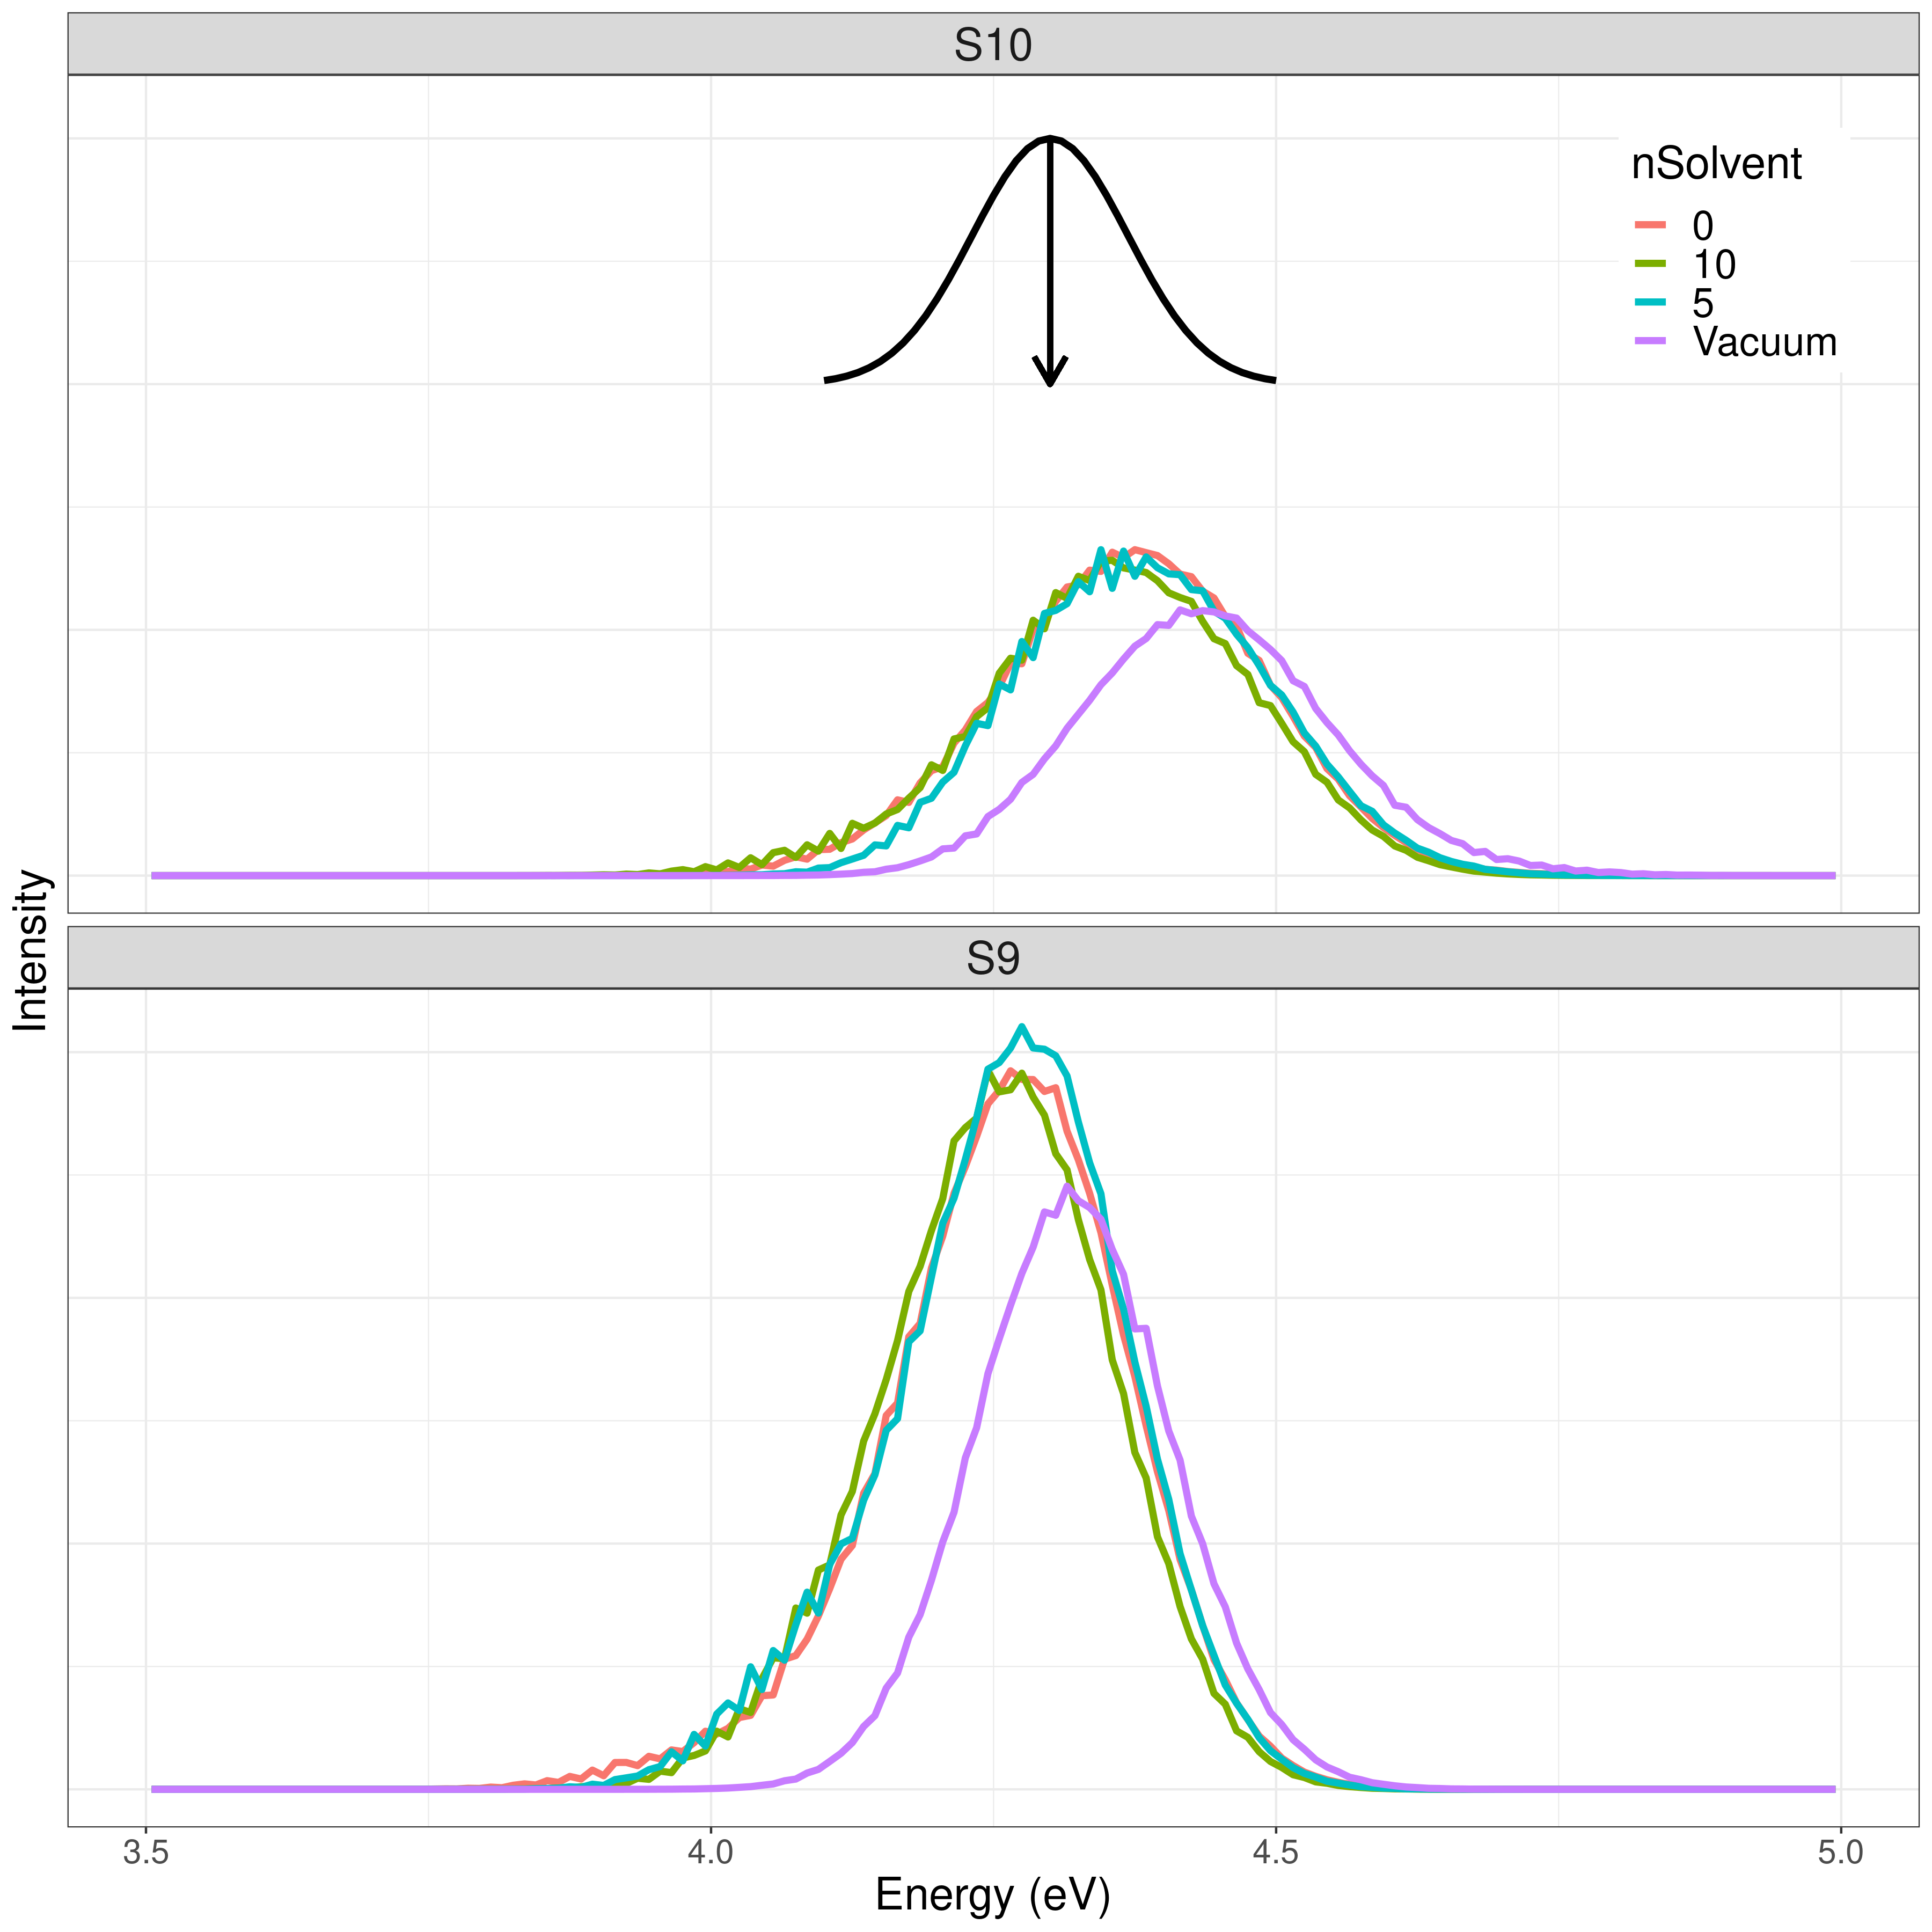
\includegraphics[width=5in]{../Paper2/Images/pulse_pump/spectra.png}
  \captionof{figure}{The calculated absorption spectrum from the first excited state S\(_1\). State energies are differences from the ground state.}
  \label{s1absorption}
\end{minipage}\bigskip

Figure \ref{s1absorption} shows the absorption spectra observerd from state S1 as energy differences from the ground state.
Spectras were normalized over both states.
The intensity of state S10 is noticeably lower than that from S9, while the peak of S9 is more aligned, as such the we expect the initial population after excitation to heavily weighed toward S9, which we see.
Spectras for varying number of solvents included in the QM region as well as vacuum are shown.
A gaussian laser wavefunction with energy of 4.3 eV with FWHM of 0.16 eV is shown above the top chart.
The presence of solvent redshift the peak absorption spectra by roughly 0.1 eV similar to what was seen in the adiabatic spectra analysis.

\subsection{State Population Relaxation}

\noindent
\begin{minipage}[c]{\textwidth}
  \centering
  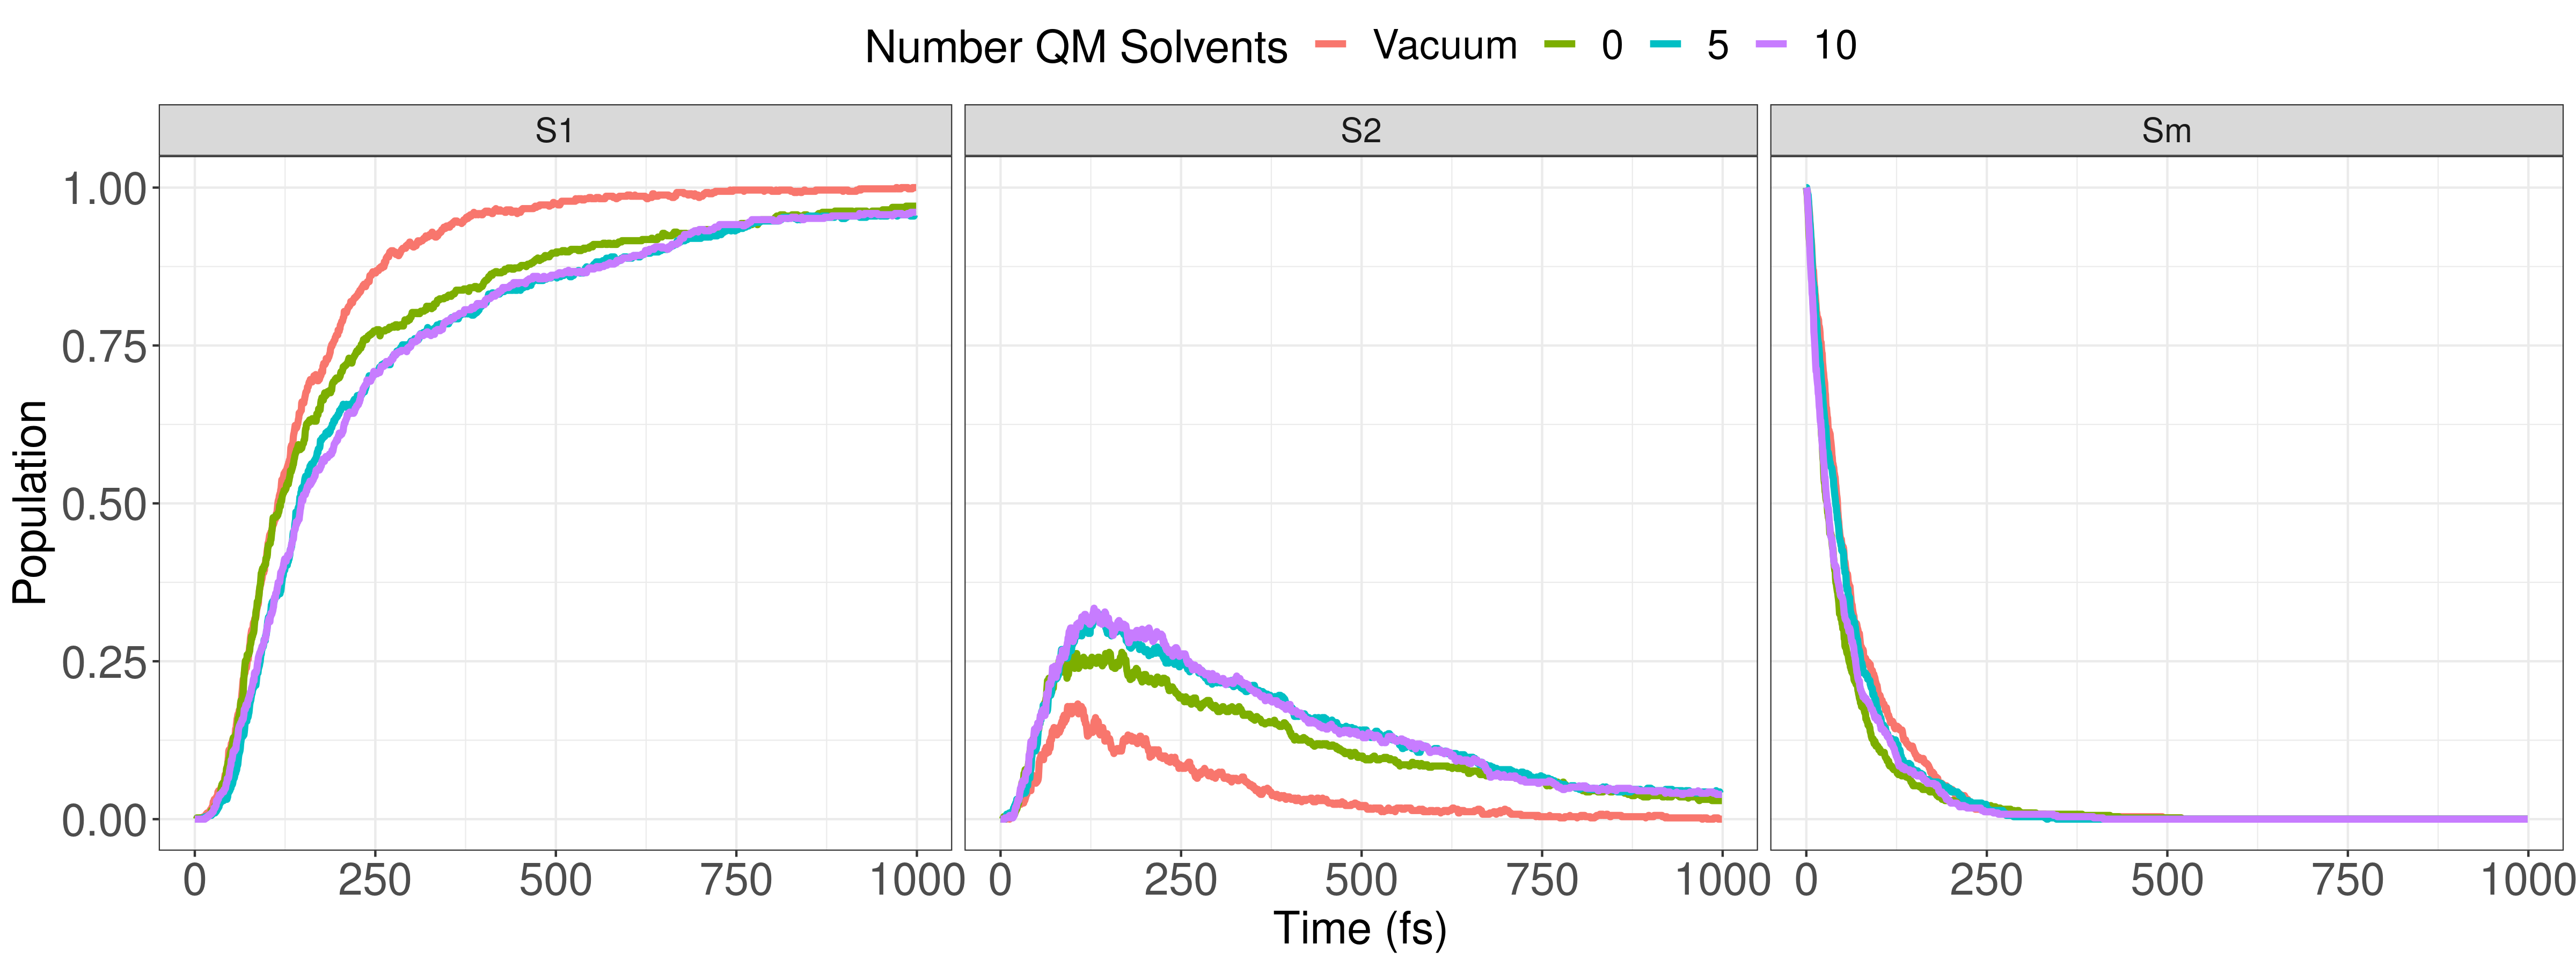
\includegraphics[width=0.9\textwidth]{../Paper2/Images/populations/solvent_comparison.png}
  \captionof{figure}{Comparison of the population decays or rises of states S\(_1\), S\(_2\), and the initial state S\(_m\) between simulations with varying number of solvents included in the QM region.}
  \label{fig:stateDecay}
\end{minipage}\bigskip

Figure \ref{fig:stateDecay} shows the population of each state calculated as
the number of trajectories at the state's potential energy surface over the
total number of trajectories. S\(_m\) represents the initial state calculated using
the pulse pump calculations previously done. States S\(_7\) and S\(_9\) are included as
the only other "slow" states, or states that reached a population of more than
0.05. The other states were excluded from the graph. These charts show that the
addition of the NO\(_2\) oligimors dramatically speed up the state relaxation. S\(_m\)
ranged from S\(_9\) to S\(_15\) for PPV\(_3\) and S\(_11\) to S\(_21\) for PPV\(_{3}\)-NO\(_{2}\). Figure
ref:fig:s1-populations, shows the rise of the S\(_{1}\) populations over the first
500 fs after excitation. We model these rises by fitting the curves to the
function
\begin{equation}
f(t) = \frac{Ae^{t/\tau}}{A+e^{t/\tau}} - \frac{A}{1+A}
\end{equation}
where $t$ is time, $\tau$ is the relaxation, and $A$ is a constant that
normalizes such that the populations remain between 0 and 1. The results are displayed in ref:table:s1. 
We clearly see that adding a test for trivial-nonavoided crossing slows the rate
of relaxation from a time constant of 258~fs. This is to be expected since we
are now preventing transitions (mostly downward) that should not occur. The
methanol have mixed results with regards to PPV3 and seem to slightly slow the
relaxation of PPV\(_3\)-NO\(_2\). Experiments using ultrafast spectroscopy have shown that
for PPV thin films the time constant for relaxations should be around 200 fs.
However, that was on thin films and for PPV\(_3\), the energy gap !! Average S\(_1\) ->
S\(_m\) energy gap) than in the thin film (0.8eV). Previous research using the
NAESMD framework have shown a time constant of 394 fs, but this was without the
test for trivial non-avoided crossings.

\subsection{Potential Energy Relaxation}

\noindent
\begin{minipage}[c]{\textwidth}
  \centering
  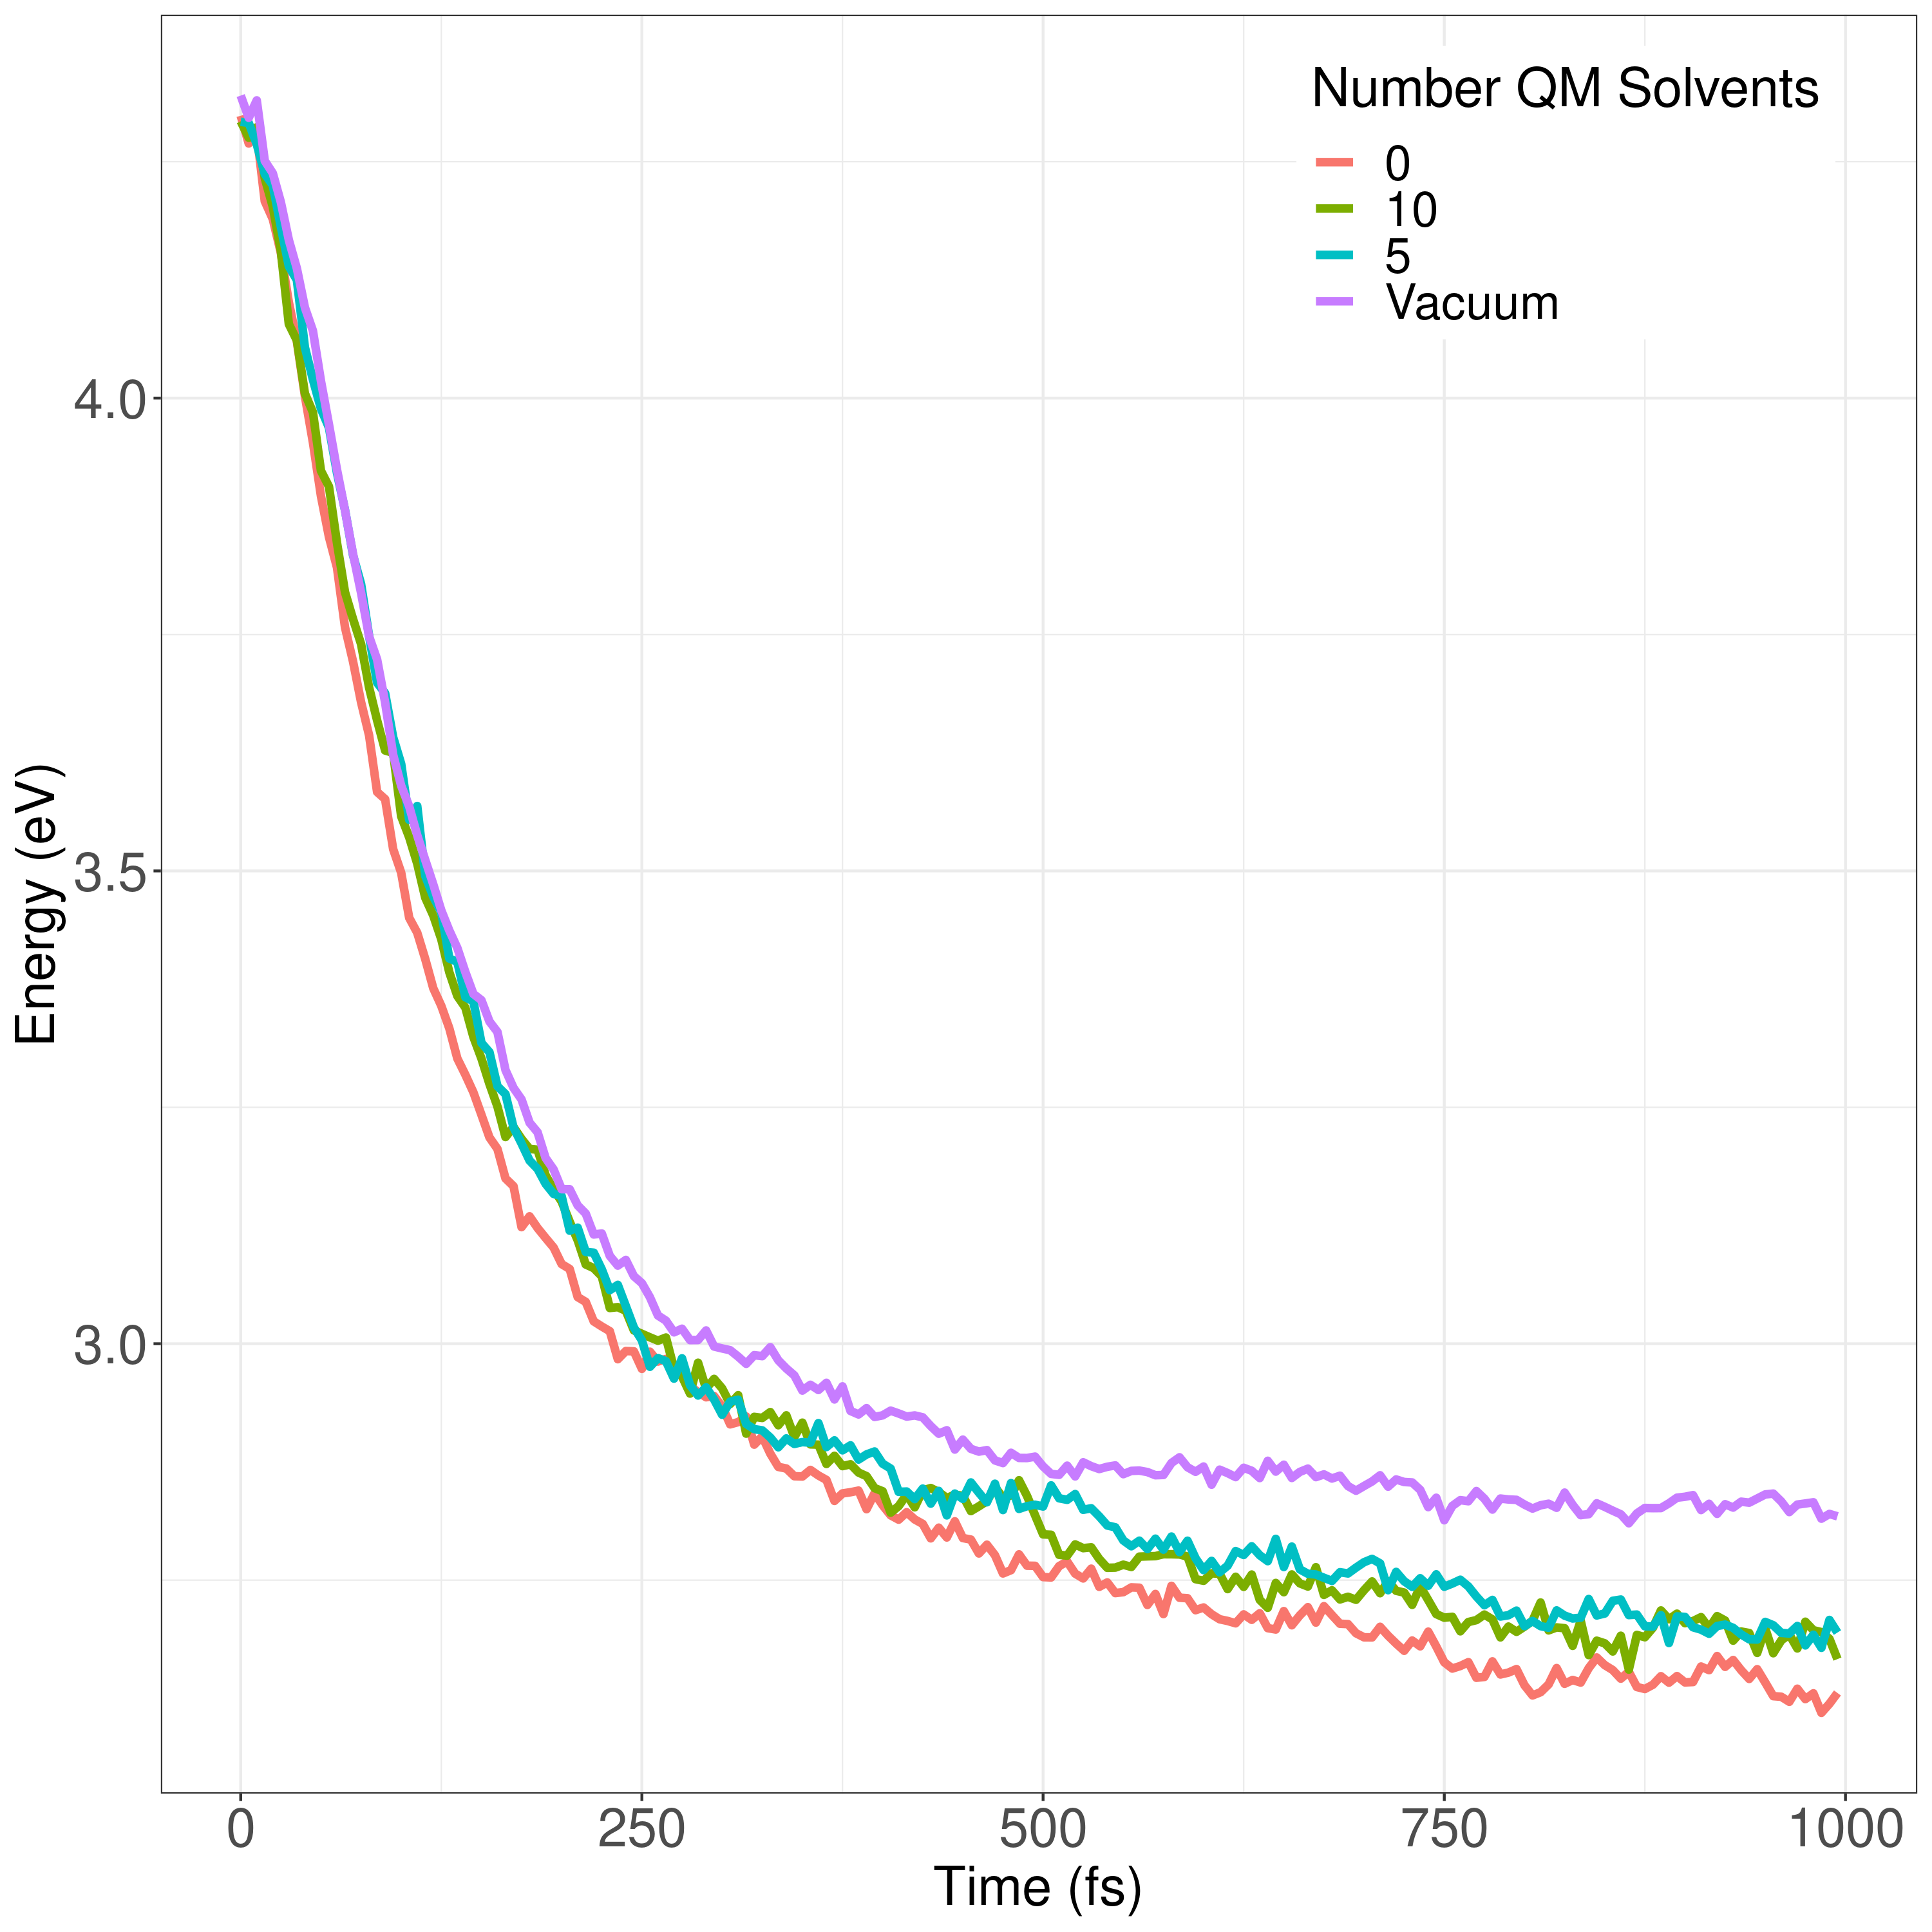
\includegraphics[width=0.5\textwidth]{../Paper2/Images/potential_energies/solvent_comparison.png}
  \captionof{figure}{Potential energy difference from the intial ground state during dynamics averaged over trajectories.}
  \label{fig:naPERelaxation}
\end{minipage}\bigskip

Figure \ref{fig:naPERelaxation} shows the ultra-fast potential engery decay average over all trajectories inside a methanol solvent with various numbers of solvent included in the QM region and vacuum.
Reported energies are in respect to the ground state energies at the initial step.
The initial relaxation rates up to aroun 100 fs, are similar in all instances.
Over time, the rate in vacuum seems to slow quicker than in solvent.
The energy in solvent also equilibrat at around 0.2 eV higher than the solvent.
No noticiable differences can be decerned between the inclusion of 5 or 10 solvents in the QM region.
Having a complete MM solvent solution seems to produce a lower energy.

\subsection{Torsional Angle Relaxation}

\noindent
\begin{minipage}[c]{\textwidth}
  \centering
  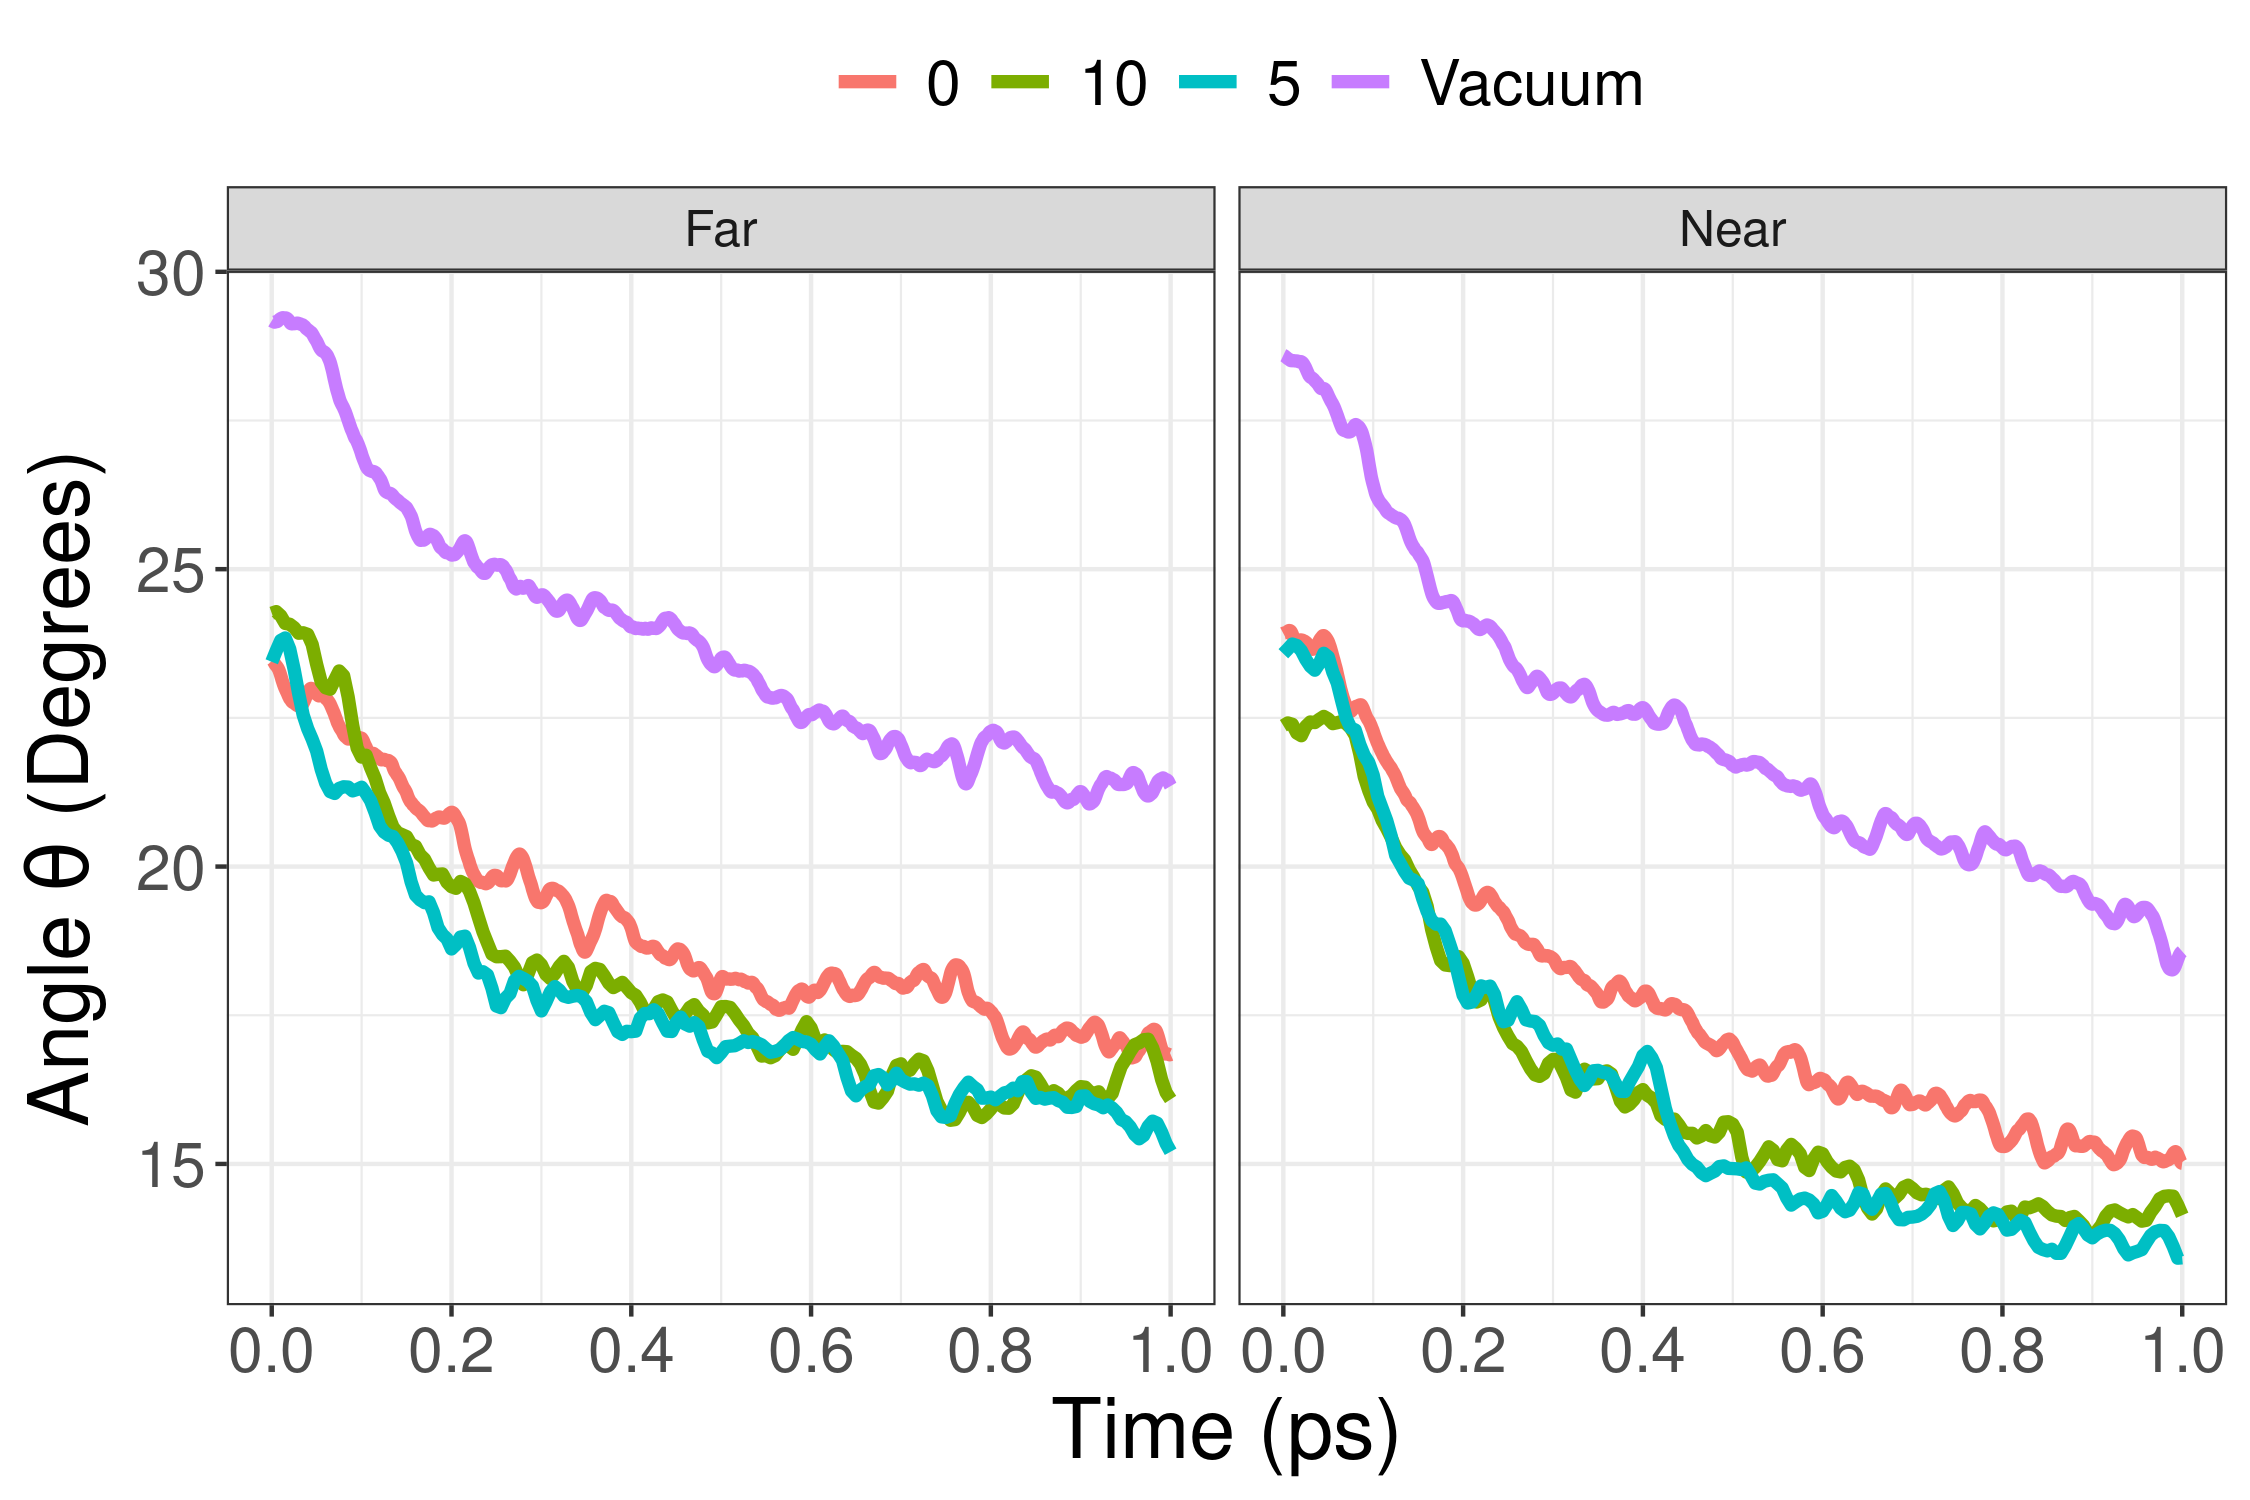
\includegraphics[width=\textwidth]{../Paper2/Images/dihedral/solvent_comparison.png}
  \captionof{figure}{Dihedral angles of PPV\(_{3}\)-NO\(_{2}\) with varying number of solvents included in the QM region.}
  \label{fig:dihedralNonadiabatic}
\end{minipage}\bigskip

Figure \ref{fig:dihedralNonadiabatic} presents the torsional angles around d1,d2,d3 (Near) and d4,d5,d6 (Far).
Similar to what was reported in the adiabatic simulations, the angles reported in vacuum remain rougly 5\(^\circ\) higher than those reported in the methanol solution.
Relaxation in the methanol solution is slightly quick than in vacuum.
Then equilibrated torsional angle in the full MM solvent could possibly be a few degrees higher than in the mixed QM/MM solvents.
Relaxations are faster, and approach a lower minimum near the nitrate group.

\subsection{Bond Length Alternation}

\noindent
\begin{minipage}[c]{\textwidth}
  \centering
  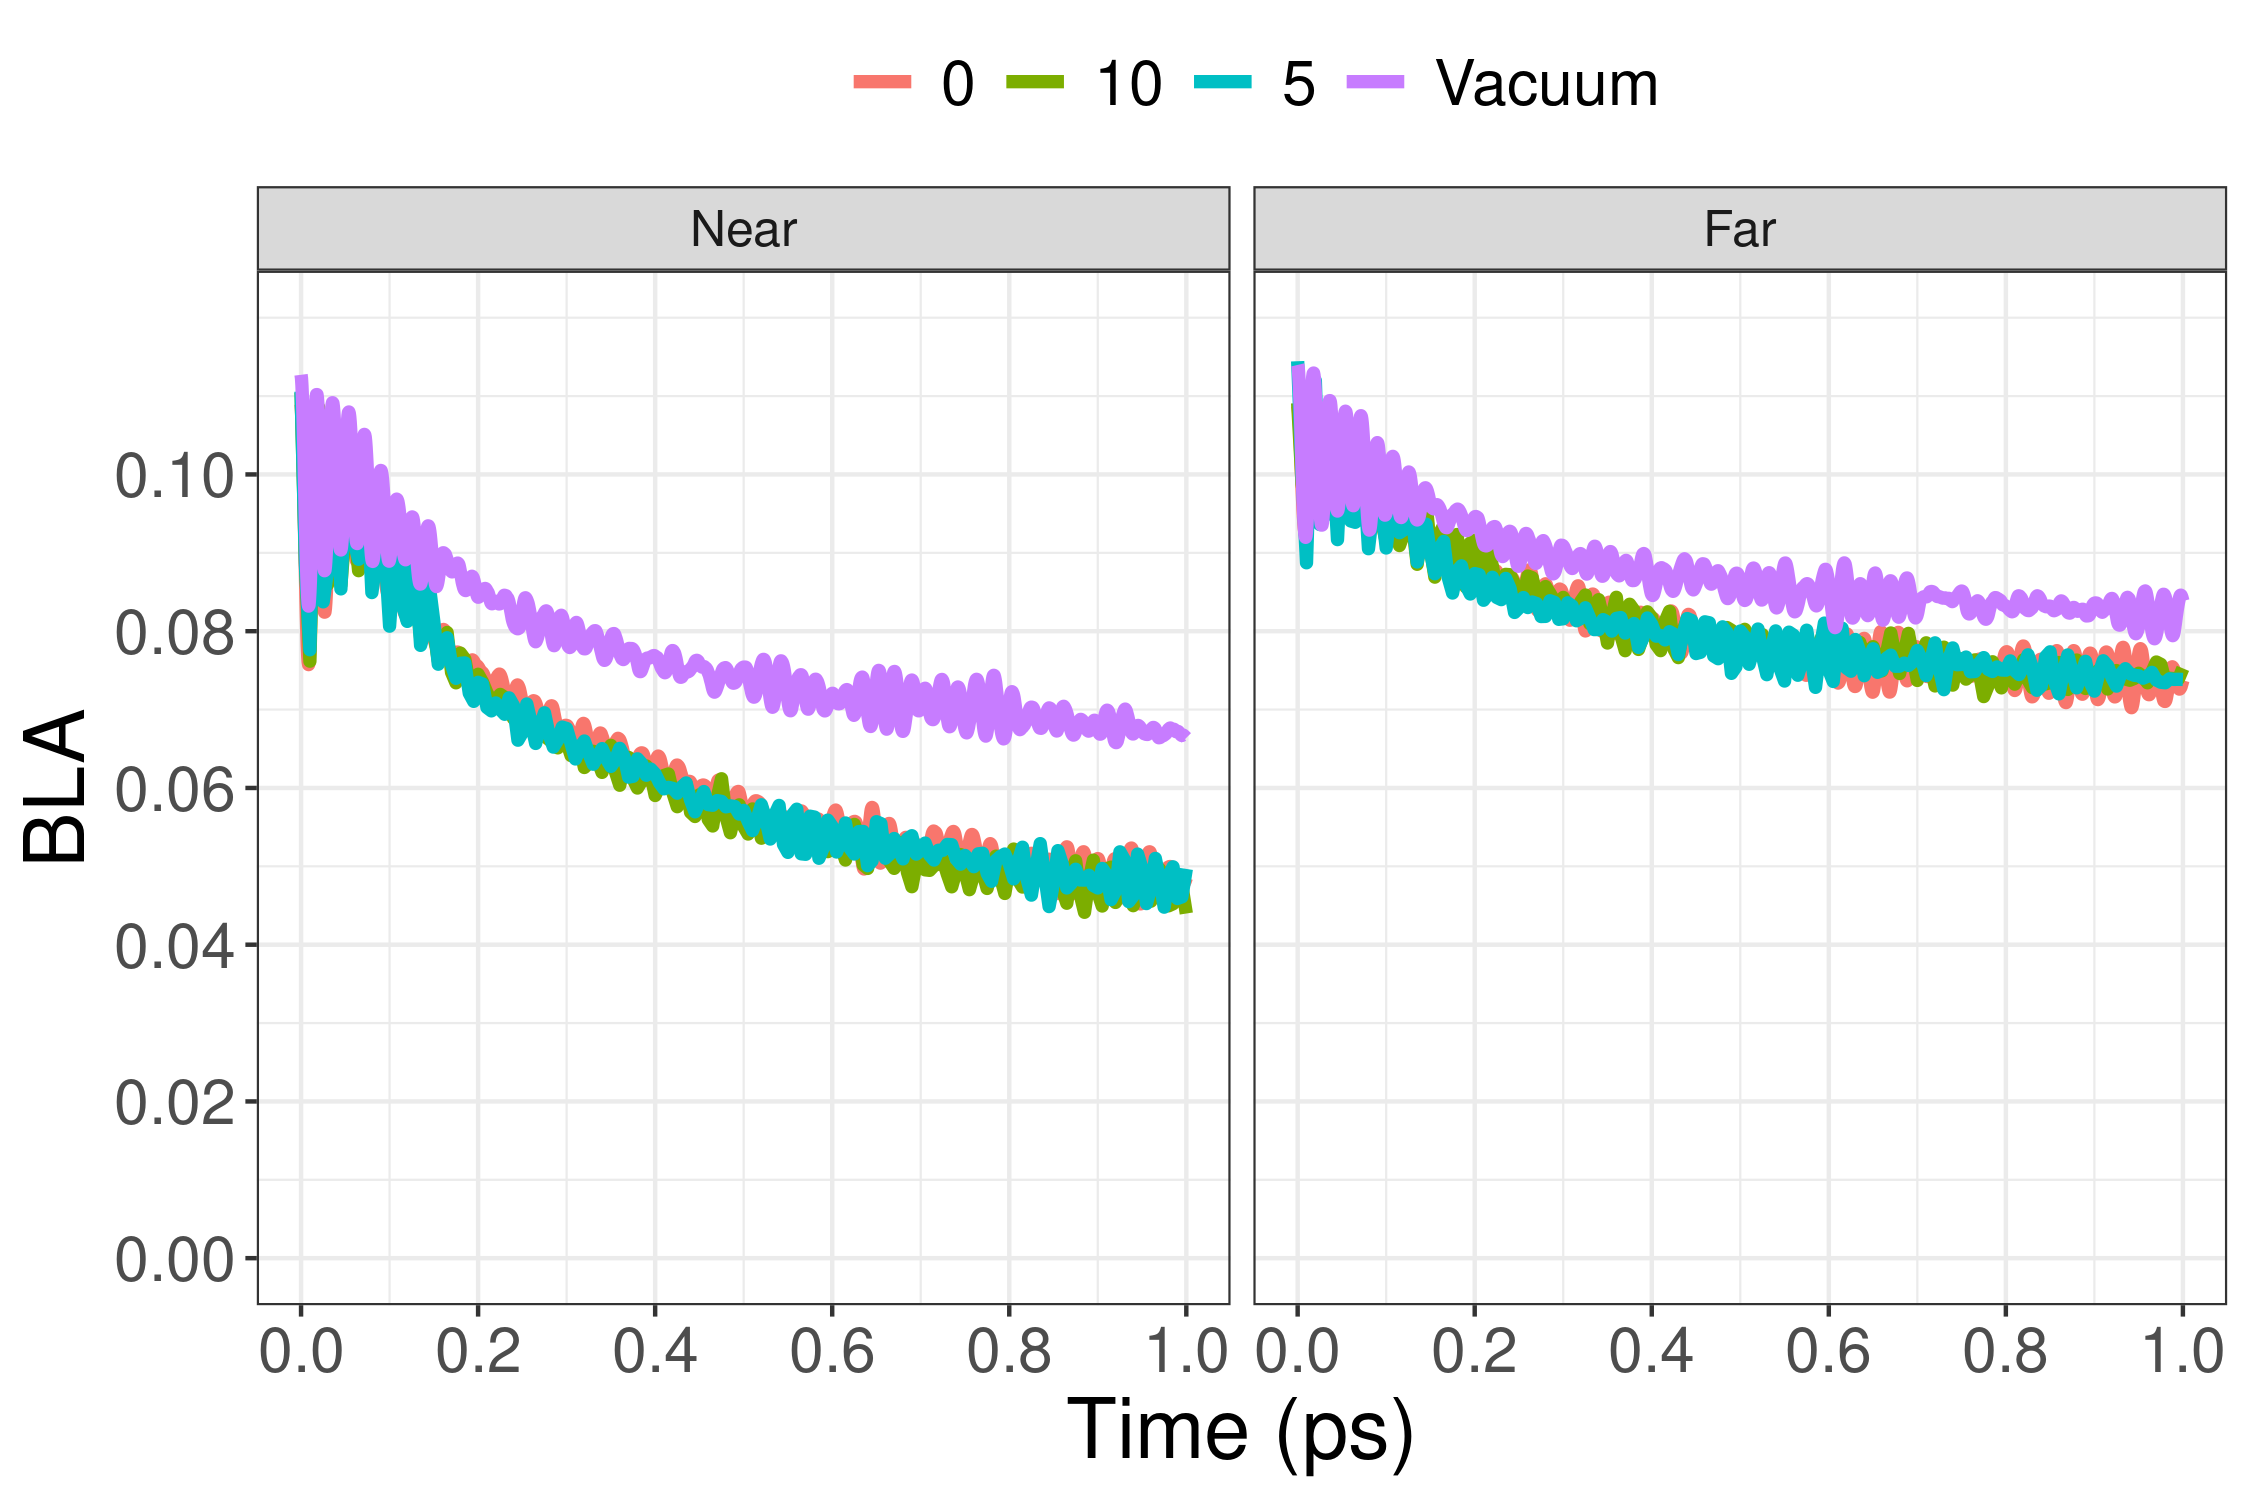
\includegraphics[width=\textwidth]{../Paper2/Images/bla/solvent_comparison.png}
  \captionof{figure}[Bond Length Alternation during Non-Adiabatic Dynamics]{The bond length alternations for bonds d1, d2, and d3 (Near) and d4, d5, d6 (Far)}
  \label{fig:naBLA}
\end{minipage}\bigskip

Figure \ref{fig:naBLA} demonstrates the variation in the bond length alternation for various number of included QM solvents and vacuum.
In all instances vacuum relaxes at a slower rate and to a higher minimum than the corresponding alternations in methanol solvent.
Relaxation are quicker and toward a lower minimum near the nitrate group.
Little discernable differences can be sceen by adding solvents to the QM region.

\subsection{Widberg Bond Orders}

\noindent
\begin{minipage}[c]{\textwidth}
  \centering
  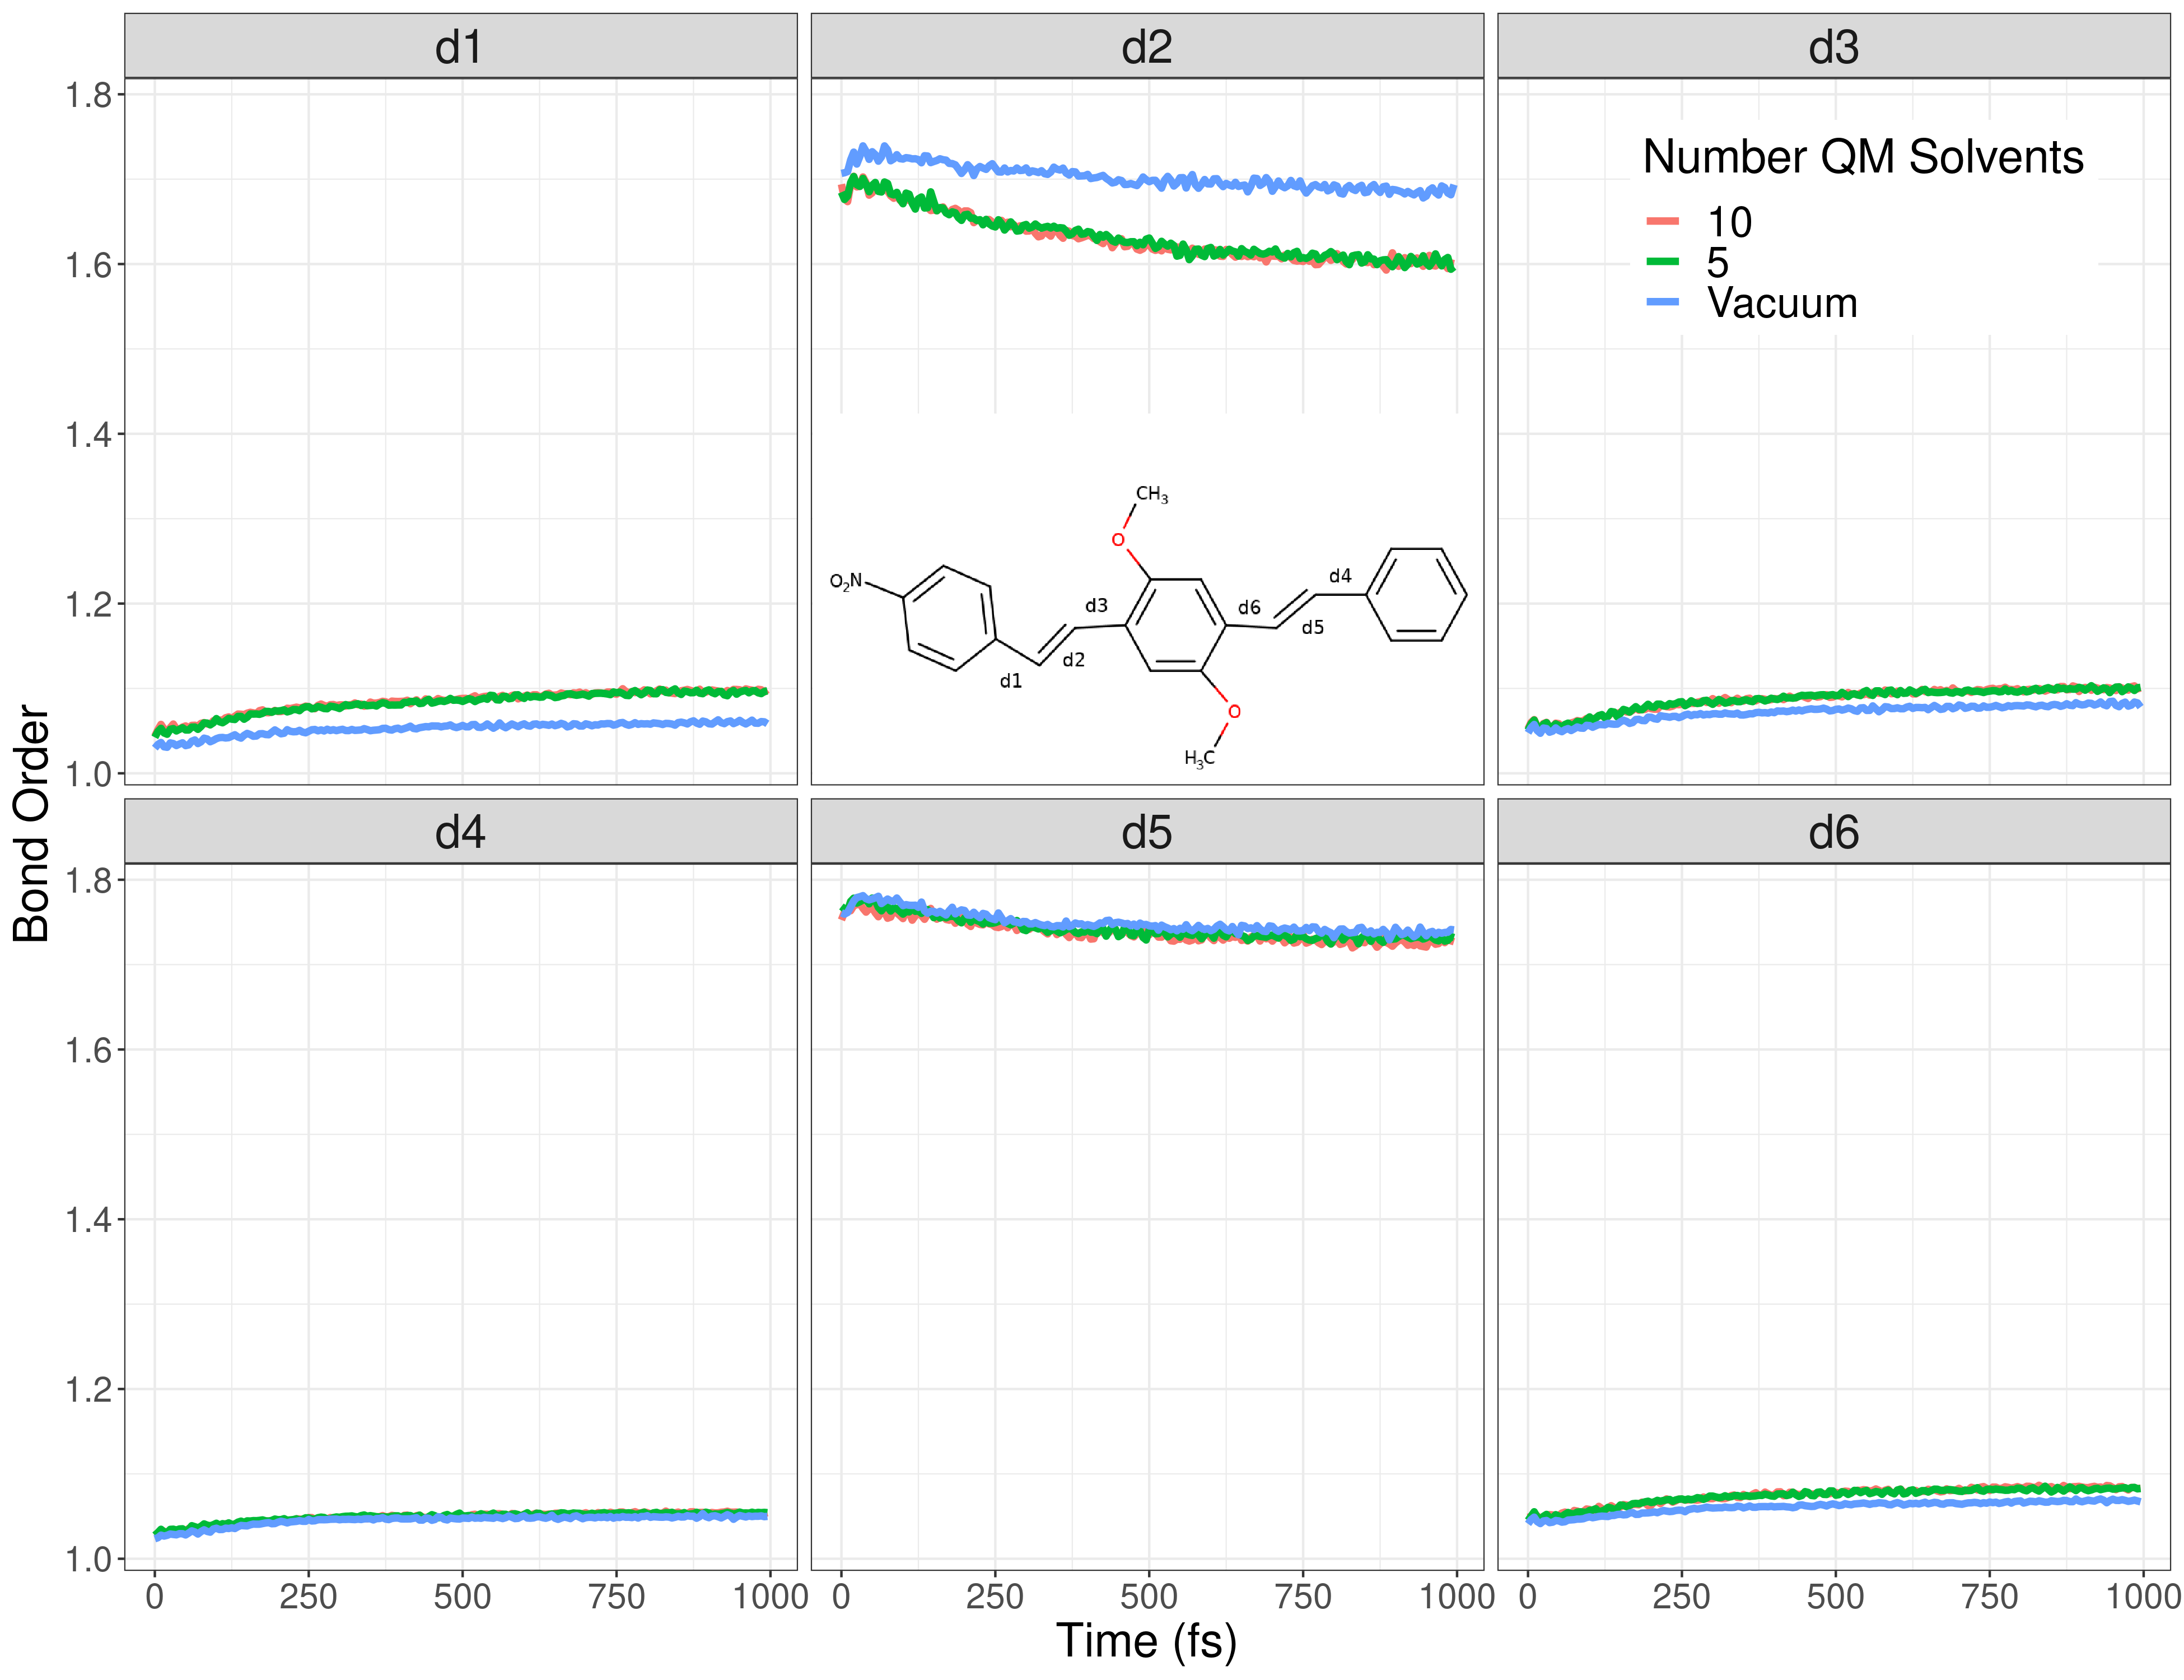
\includegraphics[width=5in]{../Paper2/Images/bond_order/solvent_comparison.png}
  \captionof{figure}[Wiberg Bond Orders in Nonadiabatic Dynamics]{The Wiberg Bond Orders averaged over the ensemble of trajectories for select bonds for PPV\(_3\)-NO\(_2\) with various number of solvents included in the QM region.}
  \label{fig:bondOrderNonadiabatic}
\end{minipage}\bigskip

The visual analysis of the Widberg bond orders can be found in figure \ref{fig:bondOrderNonadiabatic}.
The outer bonds d1,d3,d4,d6 slowly rise and gain more double bond characteristics while the inner bonds d2 and d5 lower and gain more single bond characteristics.
Little solvent effect can be descerned for the bond furthest from the nitrate group d4,d5,d6.
Noticeable solvent effects exist in the group nearest the nitrate group, with the solvent apparently amplifying the effect found in vacuum.
The inclusion of solvent in the QM region has relatively negligible effects on the bond order compared to the addition of MM solvents.
These results align well with what was found in the analysis for the bond length alternation.
